  \documentclass[twoside=false, %  doppelseitiger Druck
    DIV=15,% DIV Faktor für Satzspiegelberechnung, sie Doku zu KOMA Script
    BCOR=15mm, % Bindekorrektur
    chapterprefix=false,
    headinclude=true,
    footinclude=false,
    pagesize,%         write pagesize to DVI or PDF
    fontsize=11pt,%             use this font size
    paper=a4,%          use ISO A4
    bibliography=totoc,%         write bibliography-chapter to table of contents
    index=totoc,%         write index-chapter to table of contents
%    listof=totoc,
    cleardoublepage=plain,% \cleardoublepage generates pages with pagestyle empty
    headings=big,%       A4/B5
    listof=flat,%        improved list of tables
    numbers=noenddot
  ]{scrbook}


\usepackage{rotating} 
\usepackage{adjustbox}

\usepackage{graphicx}
\usepackage[table,xcdraw]{xcolor}

\usepackage[utf8]{inputenc}
\usepackage{makeidx}
\usepackage{amsfonts}
\usepackage[slantedGreek,sc]{mathpazo}  % Schriftart Palatino
% \usepackage{lmodern}    % statt mathpazo, falls CM Fonts verwendet werden sollen
%\usepackage{mathptmx}    % statt mathpazo, falls Times  verwendet werden soll
\usepackage[scaled=.95]{helvet}
\usepackage{courier}
\usepackage[T1]{fontenc}
\usepackage{textcomp}
\usepackage{amsmath}            % standard math notation (vectors/sets/...)
\usepackage{bm}        % standard math notation (fonts)
\usepackage{fixmath}        % standard math notation (fonts)
\usepackage{graphicx}
\usepackage[facing=yes]{floatrow}       % mehrere Gleitobjekte nebeneinander/caption neben Bild/Tabelle
\usepackage[labelfont=bf,sf,font=small,labelsep=space,format=plain]{caption}
\usepackage{subcaption}
\usepackage{scrpage2}
% \usepackage{pstool}  % einbinden falls psfrag verwendet werden soll
\usepackage{epstopdf}
\usepackage[ngerman]{babel}
\usepackage{ellipsis}  % Korrigiert den Weißraum um Auslassungspunkte
\usepackage{microtype}  % optischer Randausgleich etc.
\usepackage
{acronym}  %Abkürzungsverzeichnis
\usepackage{xcolor}         % z.B. für schattierte Boxen
\usepackage{framed}			% shaded Umgebung
\definecolor{shadecolor}{gray}{.85}%

% Links im PDF
\usepackage[colorlinks=false,
            pdfborder={0 0 0},
            breaklinks=true]
            {hyperref}

\definecolor{bluekeywords}{rgb}{0,0,1}
\definecolor{greencomments}{rgb}{0,0.5,0}
\definecolor{redstrings}{rgb}{0.64,0.08,0.08}
\definecolor{xmlcomments}{rgb}{0.5,0.5,0.5}
\definecolor{types}{rgb}{0.17,0.57,0.68}

\usepackage{listings}
\usepackage{url}
\usepackage{footmisc}
\usepackage{chngcntr}





\counterwithout{footnote}{chapter}

\renewcommand{\lstlistingname}{Beispiel}% Listing -> Algorithm
\renewcommand{\lstlistlistingname}{\lstlistingname verzeichnis}%


\lstset{language=[Sharp]C,
	captionpos=b,
	%numbers=left, %Nummerierung
	%numberstyle=\tiny, % kleine Zeilennummern
	frame=lines, % Oberhalb und unterhalb des Listings ist eine Linie
	showspaces=false,
	showtabs=false,
	breaklines=true,
	showstringspaces=false,
	breakatwhitespace=true,
	escapeinside={(*@}{@*)},
	commentstyle=\color{greencomments},
	morekeywords={partial, var, value, get, set},
	keywordstyle=\color{bluekeywords},
	stringstyle=\color{redstrings},
	basicstyle=\ttfamily\small,
}


%\typearea[current]{calc}


% Einstellungen für Bild-/Tabellenbeschriftung neben dem Bild
\floatsetup[figure]{capbesideposition={inside,top}}
\floatsetup[table]{capbesideposition={inside,top},style=plaintop}
\renewfloatcommand{fcapside}{figure}[\capbeside][\FBwidth]
\newfloatcommand{tcapside}{table}[\capbeside][\FBwidth]

\lstdefinelanguage{Gherkin}{
	keywords={When, Then, Given, And},
	ndkeywords={Feature, Scenario},
	sensitive=false,
	comment=[l]{\#},
	morestring=[b]',
	morestring=[b]"
}

\newcommand*{\quelle}{% 
	\footnotesize Quelle: 
}
\selectlanguage{ngerman}


\deffootnote{1em}{1em}{%
 \makebox[1em][l]{\thefootnotemark}}

\makeindex

\newcommand{\real}{\mathord{\mathrm{I\!R}}}

\begin{document}
\selectlanguage{ngerman}
\def\figdir{figures}
\def\tabledir{tables}

\frontmatter

\pagestyle{scrplain}
\pagestyle{empty}

\begin{titlepage}

%\sf
\raggedleft

\vspace*{-2cm}

\includegraphics{\figdir/HS_Logo_aktuell_CMYK.eps}

\vfill

\centering
\LARGE
% \vspace*{\fill}
%-----------
Fakultät für Informatik  \vspace{0.5cm}\\
\Large
Studiengang Informatik

\vspace{2cm}

\LARGE

Containers with Machine Guns
\vspace{2cm}

\Large
Marko Grgic, Peter Kurfer, Thomas Mildner, Sebastian Weißenbacher\\
WS 2017/18

\vspace{1.5cm}

\vspace{1cm}

\flushleft
 \Large
\vspace*{\fill}

%-----------
\begin{tabbing}
Datum der Abgabe: \= tt.mm.jjjj \kill
Datum der Abgabe: \> \ 22. Dezember 2017 \\
Prüfer: \> \ Herr\ Stefan Frai\\
\end{tabbing}
%-----------

\end{titlepage}

\cleardoubleemptypage


\cleardoubleemptypage
%\chapter*{Kurzfassung}
\thispagestyle{empty}

\bigskip



\noindent

\vspace*{\fill}
Schlagworte: 
Container, Docker, Gatling,

\cleardoubleemptypage

\pagestyle{scrplain}
\pagenumbering{roman}
% ---------------------------------------------------
% D-TOC.TEX zur Verwendung mit TEXPART
% (an eigene Gegebenheiten anzupassen)
% ---------------------------------------------------
%
\tableofcontents
\cleardoublepage





\pagestyle{scrheadings}


\addtokomafont{caption}{\small}

\mainmatter

\include{chapters}
\chapter*{Kurzfassung}
\thispagestyle{empty}

\bigskip



\noindent

\vspace*{\fill}
Schlagworte: 
Container, Docker, Gatling,

\chapter{Einleitung}
Das stark zunehmende Outsourcing in die Cloud beschränkt sich lange nicht mehr auf bloße Daten. Mittlerweile werden ganze Rechenzentren mit hunderten von Applikationen migriert, da es in vielen Fällen nicht mehr rentabel ist diese selbst zu hosten.
Auch die Anforderungen ändern sich mittlerweile und moderne Applikationen müssen in der Lage sein auch bei erhöhter Anzahl von Anfragen weiterhin reibungslos zu arbeiten.\\
Abhilfe dafür schafft das Cloud Buzzwort Skalierung, frei nach dem Motto \textit{viel hilft viel}. Heute laufen Anwendungen häufig in einem Cluster der dynamisch auf sich ändernde Anforderungen reagieren kann. Erhöht die Anzahl der Anfragen, so werden im Cluster einfach neue Instanzen der Applikation gestartet um die gestiegene Last verarbeiten zu können und werden danach wieder heruntergefahren.
\\\\
Doch wie testet man ob die Anwendung schnell genug skaliert, wie viele Anfragen hält sie aus, bei welcher Last bricht sie doch ein?\\
Dafür gibt es verschiedene Tools für Lasttests, eines davon ist Gatling.\\
Gatling ermöglicht es einem Testszenarios zu entwerfen, um damit die gewünschte Applikation immer wieder unter den gleichen Bedingungen unter Last zu setzen und zu messen wie diese darauf reagiert.\\
Ziel dieser Projektarbeit war es, die Skalierbarkeit die die Cloud für Container-Anwendungen bringt, auch auf das Tool für Lasttests anzuwenden. Zum einen, um dieses unabhängig von einer konkreten Plattform betreiben zu können, zum anderen, um die maximal erzeugte Last erhöhen zu können wenn auch der Lasttest im Cluster läuft. Siehe \textit{viel hilft viel}.\\\\
In den nächsten Kapitel werden durch Einführung in Docker und Gatling die für das Verständnis nötigen Grundlagen geschaffen, sowie Kubernetes als Beispiel für ein Tool zum Management von Container Clustern vorgestellt. Danach werden die Container mit dem Gatling Maschinengewehr bestückt und eine kleine Demo Applikation unter Last gesetzt um das Ergebnis der Projektarbeit anhand eines konkreten Testfalls zu zeigen. Die Resultate der verschiedenen Testkonfigurationen werden anschließend gegeneinander verglichen, um ein Fazit daraus ziehen zu können.\\
Als Abschluss dieser Arbeit wird noch ein kurzer Ausblick gegeben, welche Schritte vorgenommen werden können, um die Applikation für den Betrieb im Cluster zu optimieren.

\chapter{Docker}
\label{c:docker}

Zu Beginn ist es notwendig, die Grundlagen von Docker zu verstehen.
Hierfür bietet dieses Kapitel einen Einblick in die wichtigsten Begrifflichkeiten, die Architektur und die für diese Arbeit notwendigen Funktionalitäten.
Falls nicht anders gekennzeichnet basiert dieses Kapitel auf der offiziellen Dokumentation von Docker \cite{Docker:online1}.

\section{Einführung in Docker}
\label{c:einführung}

\begin{figure}
	\centering
	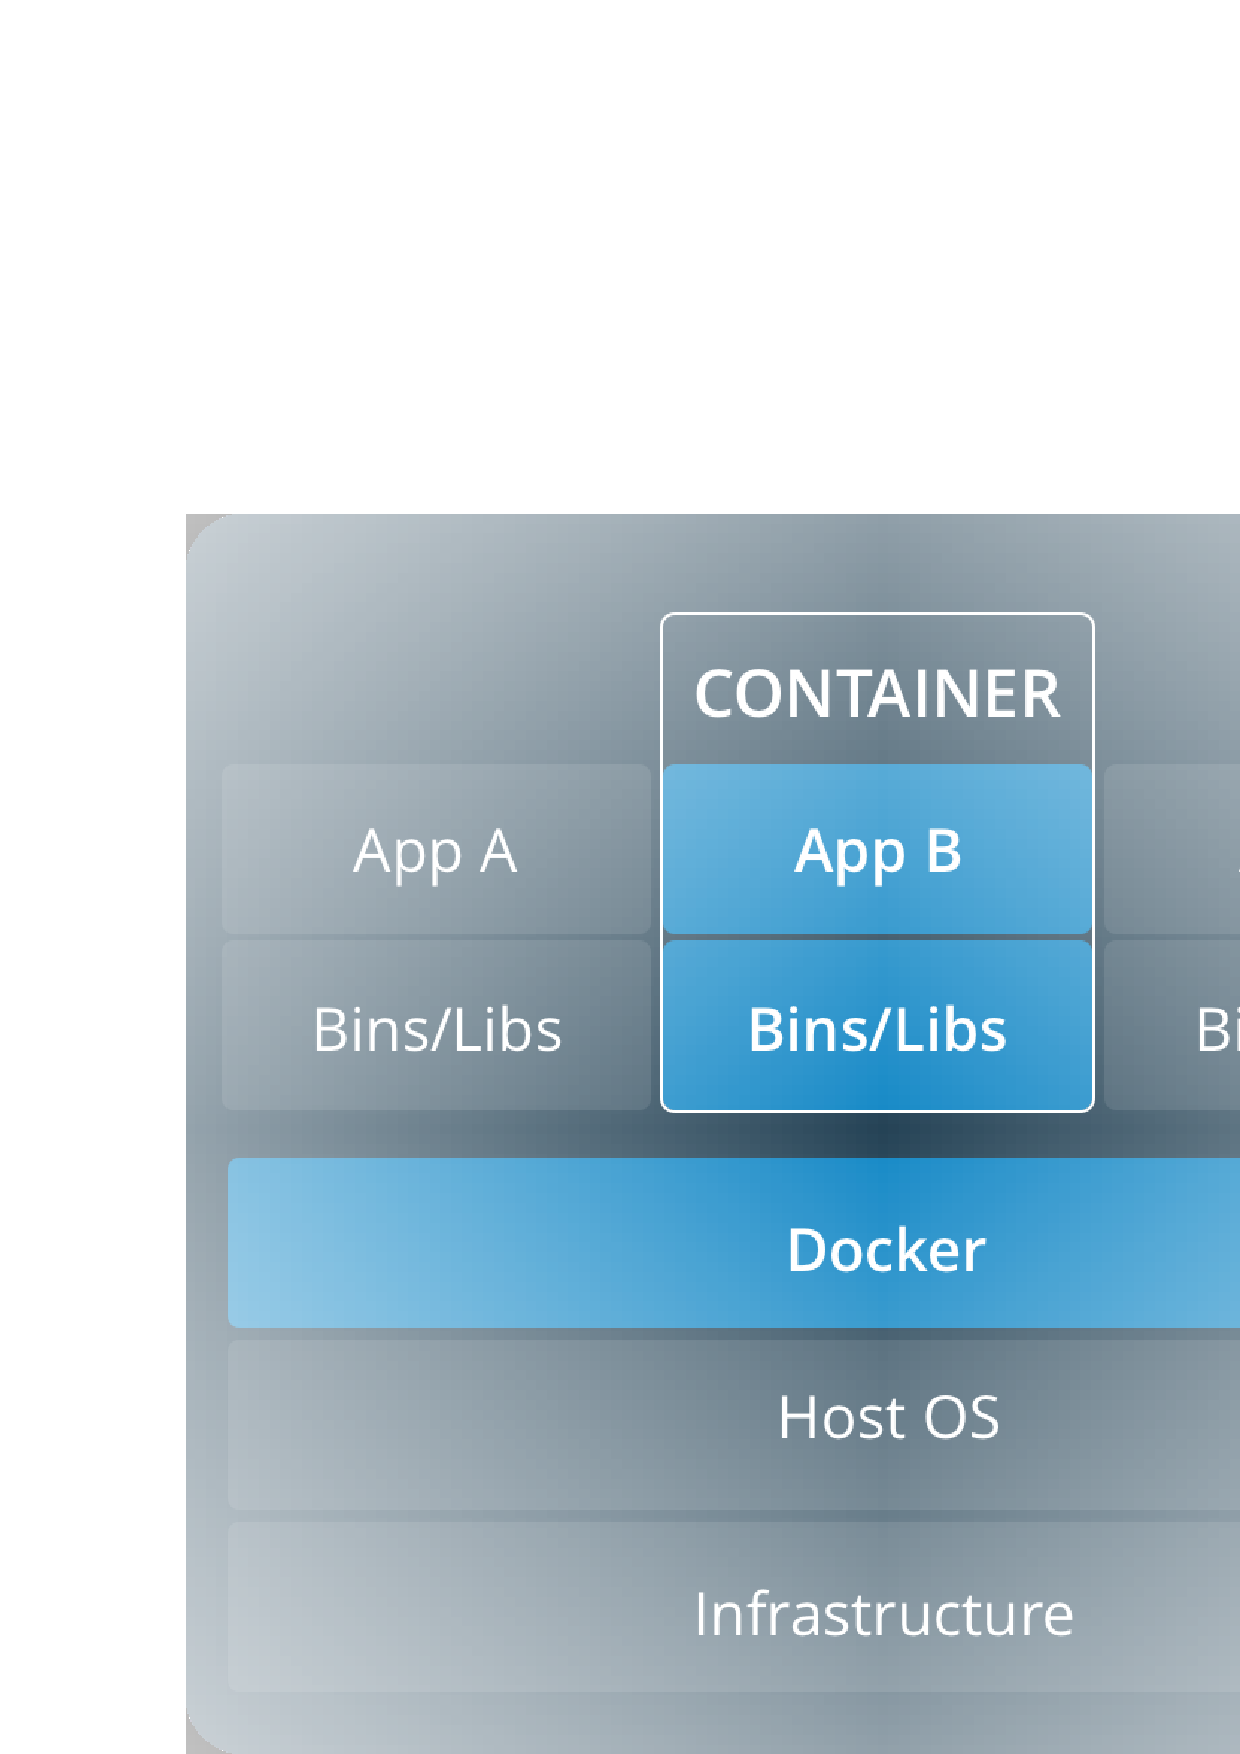
\includegraphics[width=0.7\linewidth]{figures/Docker}
	\caption[Betriebssystem basierte Virtualisierung mit Docker-Containern]{Umsetzung einer Betriebssystem basierten Virtualisierung mit Docker-Containern}
	\label{fig:docker}
	\tiny{\quelle\url{https://www.docker.com/what-container}}
\end{figure}

\begin{figure}
	\centering
	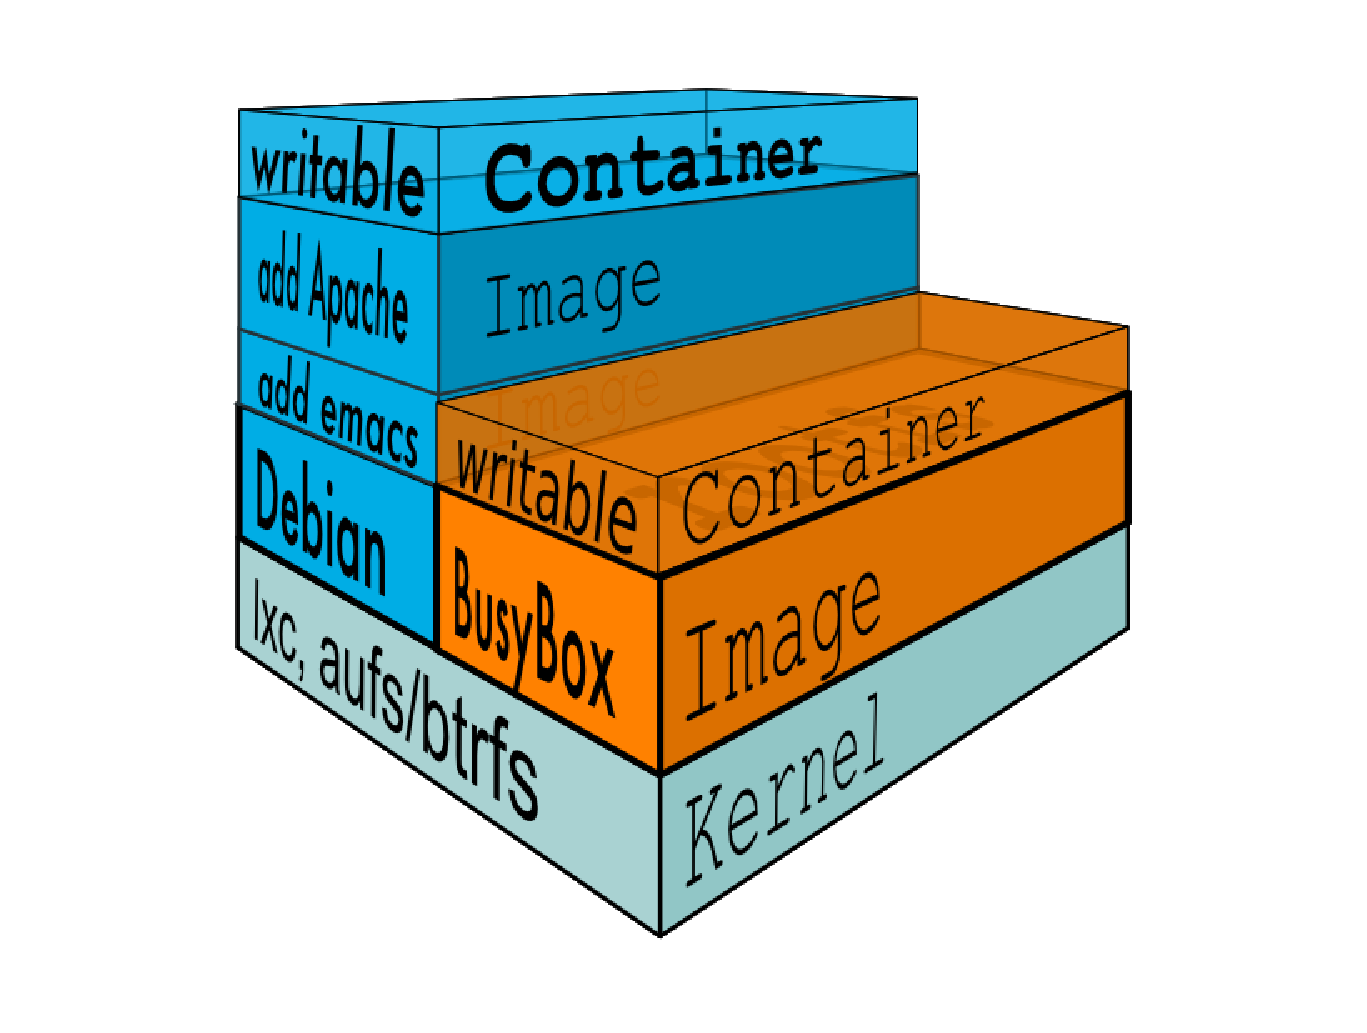
\includegraphics[width=0.7\linewidth]{figures/DockerLayer}
	\caption[Aufbau von Docker mittels Schichten]{Aufbau von Docker mittels Schichten}
	\label{fig:dockerlayer}
	\tiny{\quelle\url{https://blog.docker.com/2015/10/docker-basics-webinar-qa/}}
\end{figure}

Bei Docker handelt es sich um eine containerbasierte Virtualisierung.
Es ist möglich, die Docker-Container sowohl auf einem Windows-System, Unix-System, in der Cloud oder sogar in einer virtuellen Maschine auszuführen.
Hierfür wird, wie in Abbildung \ref{fig:docker} gezeigt, in einem Host Betriebssystem die Docker Runtime zur Verfügung gestellt sowie mehrere Docker-Container ausgeführt.
Die Docker Runtime übernimmt die Verwaltung der einzelnen Docker-Container, die die benötigten Binaries, Bibliotheken und Anwendungen enthalten.

Im Vergleich zur Virtualisierung mittels einer \ac{VM} bieten Docker-Container einige Vorteile.
Hierzu zählen einerseits der geringere Bedarf an CPU und RAM sowie andererseits die schnelle Startgeschwindigkeit eines Docker-Containers im Vergleich zu einer herkömmlichen \ac{VM}.

Trotz dessen, dass sich die Docker-Container, wie in Abbildung \ref{fig:docker} abgebildet, einen Betriebssystemkernel teilen, sind diese vollständig voneinander isoliert, was dazu führt, dass sich Docker-Container besonders für Continuous Integration und Development eignen.
Dies ist möglich, da die Workspaces, in Docker \glqq{}Container\grqq{} genannt, auf Linux Containern basieren und somit zur Isolierung die folgenden Namespaces genutzt werden:

\begin{itemize}
	\item \textit{ipc}-Namespace zur Verwaltung der Interprozess Kommunikationsressourcen (Shared Memory)
	\item \textit{mnt}-Namespace zur Verwaltung des Dateisystems
	\item \textit{net}-Namespace zur Verwaltung des Netzwerk Interfaces
	\item \textit{pid}-Namespace zur Isolation von Prozessen
	\item \textit{uts}-Namespace zur Isolation des Kernels und der Versions Identifier
\end{itemize}

Zur Kontrolle der Hardware Ressourcen verwendet Docker die von Linux stammenden \ac{cgroups}.
Mittels dieser ist es möglich, den Containern Hardware Ressourcen zuzuweisen und diese nötigenfalls, wie z. B. den RAM, zu beschränken.

Neben den oben genannten Funktionen nutzt Docker mit dem \ac{UnionFS} eine weitere Linux Funktion.
Hierbei wird, wie in Abbildung \ref{fig:dockerlayer} zu sehen, auf dem Boot Dateisystem (Kernel) ein Dateisystem Stack erzeugt, der aus mehreren read-only Layern, die Images genannt werden, besteht.
Jedes Image referenziert und beinhaltet lediglich Ergänzungen zum vorherigen Image.
Dies macht Docker leichtgewichtig und schnell und ermöglicht einen im Vergleich zu traditionellen \acp{VM} höheren operativen Workload auf der gleichen Hardware.

Beim Start von Docker wird, wie in Abbildung \ref{fig:dockerlayer} dargestellt, ein read-write Layer auf dem Stack erzeugt.
In diesen werden die notwendigen Dateien der darunterliegenden Images kopiert (\textit{copy-on-write}), dort nötigenfalls umgeschrieben und abgelegt.
Wird Docker gestoppt, so wird der writable Layer und damit auch sämtliche Änderungen an den Dateien gelöscht, falls nicht ein Speichervolumen außerhalb des \ac{UnionFS} angebunden wurde.
Somit ist es möglich, die Docker-Container immer zu den gleichen Bedingungen zu starten.

\section{Architektur}
\label{c:architektur}

Wird die Docker Architektur betrachtet, so zeigt die Abbildung \ref{fig:dockerengine}, dass es sich bei der Docker Runtime oder auch Docker-Engine lediglich um eine Client-Server-Architektur mit mehreren Hauptkomponenten handelt.

Im Kern der Docker-Engine befindet sich, wie in Abbildung \ref{fig:dockerengine} gezeigt, der Server oder auch Docker Daemon.
Dieser erstellt und verwaltet einerseits die Docker-Container, Images, Netzwerke und Dateisysteme und er ist andererseits in der Lage, mit anderen Docker Daemons zu kommunizieren.
Mittels einer REST-API und dem \ac{CLI} ist der Client im Stande, mit einem oder mehreren Docker Daemons zu interagieren und diesen, per \ac{CLI} Kommandos oder mit Hilfe von Skripten, Aufträge zu erteilen.

Ein weiterer wichtiger Bestandteil der Docker Architektur sind, wie in Abbildung \ref{fig:dockerarchitecture} zu sehen, die Docker Registries.
Hierbei wird zwischen privaten und öffentlichen Registries unterschieden.
Die wichtigsten öffentlichen Registries sind der Docker Hub und die Docker Cloud.
So wird z. B. mittels der Befehle \textit{docker run} oder \textit{docker pull} per default das Standard Image vom Docker Hub genutzt, um den Container über dem Dateisystem Stack automatisch zu bauen.

Jedes Image in einer Docker Registry verfügt über einen sogenannten \textit{Tag}.
Das Standard Image wird markiert durch den Tag \textit{latest}.
Durch Tags ist es möglich unterschiedliche Versionen eines Containers unter dem selben Namen zu gruppieren.
Beispielsweise gibt es den offiziellen Java-Container sowohl mit JDK 7, 8 oder 9 und mit JRE 7, 8 oder 9.

Des Weiteren besteht die Möglichkeit, mit Hilfe des \ac{DDC} eigene (private) Registries anzulegen und z. B. mittels des \textit{docker push} Kommandos eigene Images in den neu angelegten Registries abzulegen und später für den Buildprozess zu nutzen.

\begin{figure}
	\centering
	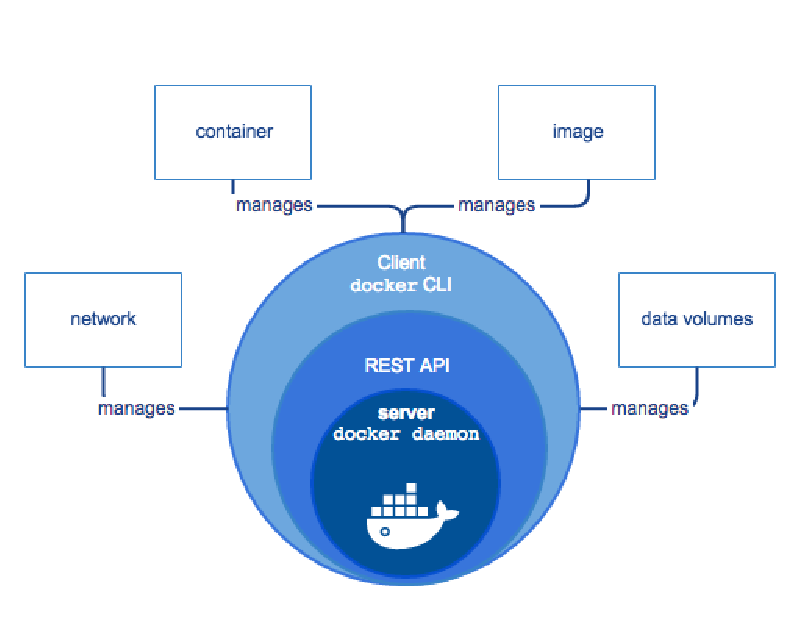
\includegraphics[width=0.7\linewidth]{figures/DockerEngine}
	\caption[Aufbau Docker-Engine]{Schematische Darstellung des Aufbaus der Docker-Engine}
	\label{fig:dockerengine}
	\tiny{\quelle\url{https://docs.docker.com/engine/docker-overview/}}
\end{figure}

\begin{figure}
	\centering
	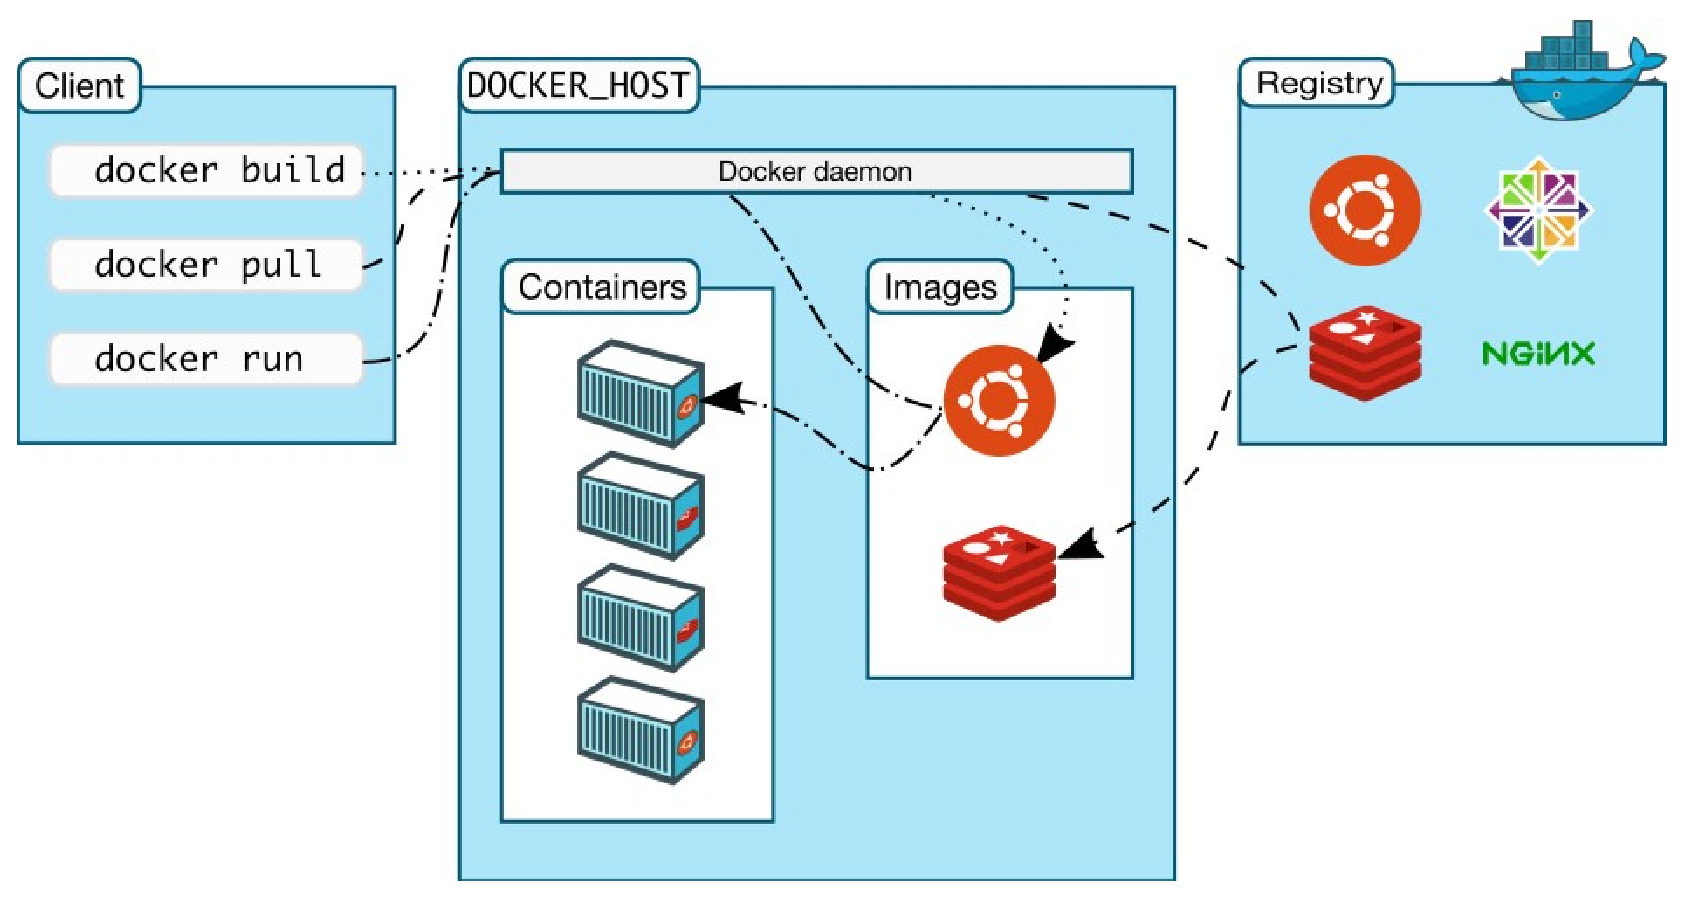
\includegraphics[width=0.7\linewidth]{figures/DockerArchitecture}
	\caption[Detailansicht der Docker-Architektur]{Detailansicht der Docker-Architektur}
	\label{fig:dockerarchitecture}
	\tiny{\quelle\url{https://docs.docker.com/engine/docker-overview/}}
\end{figure}

\section{Docker Funktionalitäten}
\label{c:funktionalität}

Im folgenden Unterkapitel werden die für diese Arbeit wichtigsten Docker Funktionalitäten erläutert.
Hierbei wird, falls notwendig anhand einer Begründung erklärt, weshalb eine bestimmte Ausprägung einer Funktionalität gewählt wurde.

\subsection{Docker-Compose}
\label{ss:dockerCompose}

Standardmäßig wird jeder Docker-Container einzeln mit dem Kommando \textit{docker run} erstellt und ausgeführt.
Betrachtet man den Titel dieser Arbeit, "Containers with Machine Guns", so geht daraus hervor, dass es sich nicht zwingend um einen einzelnen Container handelt, sondern möglicherweise um eine Vielzahl von Containern.
Diese sollen nach Möglichkeit alle gleichzeitig gestartet und ausgeführt werden.

Um dies zu erreichen, bietet Docker Docker-Compose an.
Hierbei handelt es sich um ein Tool von Docker, mit dem es möglich ist, einen Service für eine Anwendung zu konfigurieren und diese sowie die dazugehörigen Container anschließend mit einem einzigen Befehl zu starten.

Hierfür wird zu Beginn ein Dockerfile erstellt, mit dem es möglich ist, die Images und Container einfach zu vervielfältigen.
Im Anschluss daran wird die YAML-Datei docker-compose.yml genutzt, um den Service zu definieren.
Code-Beispiel \ref{dockerComposeFile} zeigt, wie in dieser Datei z. B. die zwei Services \textit{web} und \textit{redis} definiert werden.
Des Weiteren wird dargestellt, wie der Service \textit{web} im Punkt \textit{build} das Dockerfile aus dem aktuellen Verzeichnis und der Service \textit{redis} das öffentliche Redis Image \glqq{}redis:alpine\grqq{} des Docker Hub verwendet.
Zusätzlich ist ersichtlich, dass der Service \textit{web} über den Default-Port 5000 des Flask Web-Servers erreichbar ist.
Mittels des Kommandos \textit{docker-compose up} wird anschließend die gesamte Anwendung anhand der Docker-Compose-Datei gestartet.

\begin{minipage}{\linewidth}
	\begin{lstlisting}[frame=single,caption=Beispiel Docker Compose Datei \cite{Docker:online2}, label=dockerComposeFile, language=Scala]
	version: '3'
	services:
	  web:
	    build: .
	    ports:
	     - "5000:5000"
	  redis:
	    image: "redis:alpine"
	\end{lstlisting}
\end{minipage}

Mit Hilfe von Docker-Compose ist es neben dem Starten des Service möglich, diesen zu stoppen, erneut zu bauen und Befehle an einzelne Container des Service zu senden.
Des Weiteren ermöglicht Docker-Compose die Statusabfrage sowie das Auslesen von Logs eines laufenden Service.

\subsection{Netzwerke}

Dieser Abschnitt des Kapitels zeigt die default Netzwerke und die Möglichkeiten zum Definieren eines eigenen Netzwerkes in Docker auf.
Hiermit soll erläutert werden, wie der angelegte Service außerhalb des Host-Systems verfügbar gemacht wird.

\subsubsection{Default Netzwerke}

Mit der Installation von Docker werden standardmäßig die folgenden drei Netzwerke erzeugt:

\begin{itemize}
	\item None-Netzwerk
	\item Host-Netzwerk
	\item Bridge-Netzwerk
\end{itemize}

Das None-Netzwerk ermöglicht es, einen Container zu einem spezifischen Netzwerk Stack hinzuzufügen, allerdings besitzt dieser Container kein eigenes Netzwerk-Interface. 
Mit Hilfe des Host-Netzwerkes wird der Container zum Netzwerk Stack des Host Systems hinzugefügt.
Dies hat zur Folge, dass keine Isolation zwischen dem Host System und den Containern mehr gegeben ist.
Des Weiteren sind sowohl das None als auch das Host-Netzwerk nicht direkt mit Docker konfigurierbar.

Das dritte default Netzwerk, das Bridge-Netzwerk, ist auf allen Host Systemen von Docker vorhanden.
Wird kein alternatives Netzwerk definiert, so wird jeder neu erstellte Container automatisch an dieses gekoppelt.
Die angebundenen Container wären zwar durch \textit{Port Mapping} und mit Hilfe von IP-Adressen, aber nicht mit den Container-Namen, die mittels des \ac{DNS} aufgelöst werden, in der Lage, miteinander zu kommunizieren. Dieses Vorgehen wird jedoch nicht für das default Bridge-Netzwerk von Docker empfohlen.
Stattdessen sollte für derartige Anwendungsfälle das, im Abschnitt User definierte Netzwerke, beschriebene Bridge-Netzwerk verwendet werden.

\subsubsection{User definierte Netzwerke}

Zur Erstellung eines User definierten Netzwerks bietet Docker entsprechende Treiber an.
Mit diesen ist es möglich, die folgenden Netzwerke anzulegen:

\begin{itemize}
	\item User definierte Bridge-Netzwerke
	\item Overlay-Netzwerke
	\item MACVLAN-Netzwerke
\end{itemize}

Wenn keines der gelisteten Netzwerke dem Anwendungsfall entspricht, so besteht die Möglichkeit, ein eigenes Plugin für einen Netzwerk-Treiber zu erstellen.
Eine genaue Beschreibung hierfür sowie für das oben gelistete MACVLAN-Netzwerk würde für diese Arbeit zu weit gehen, weshalb diese an dieser Stelle nur zum Zweck der Vollständigkeit erwähnt werden.

Das User definierte Bridge-Netzwerk bietet mit Hilfe des eingebetteten \ac{DNS}-Server des Docker Daemon eine \ac{DNS}-Auflösung.
Des Weiteren besteht optional die Möglichkeit zur Steuerung der Kommunikation der sich auf einem Host-System und in einem Netzwerk befindlichen Container.
Diese können an kein oder jederzeit, auch während der Ausführung eines Containers, an ein oder mehrere Netzwerke angeschlossen oder von diesen getrennt werden.
Ist dies nicht erforderlich, so sind alle Container ohne weitere Konfiguration in der Lage, mit jedem beliebigen Container des Netzwerkes zu kommunizieren.
Hieraus geht hervor, dass das Netzwerk die darin befindlichen Container vollständig, wie in Abbildung \ref{fig:dockerportpuex} zu sehen, isoliert.

\begin{figure}[H]
	\centering
	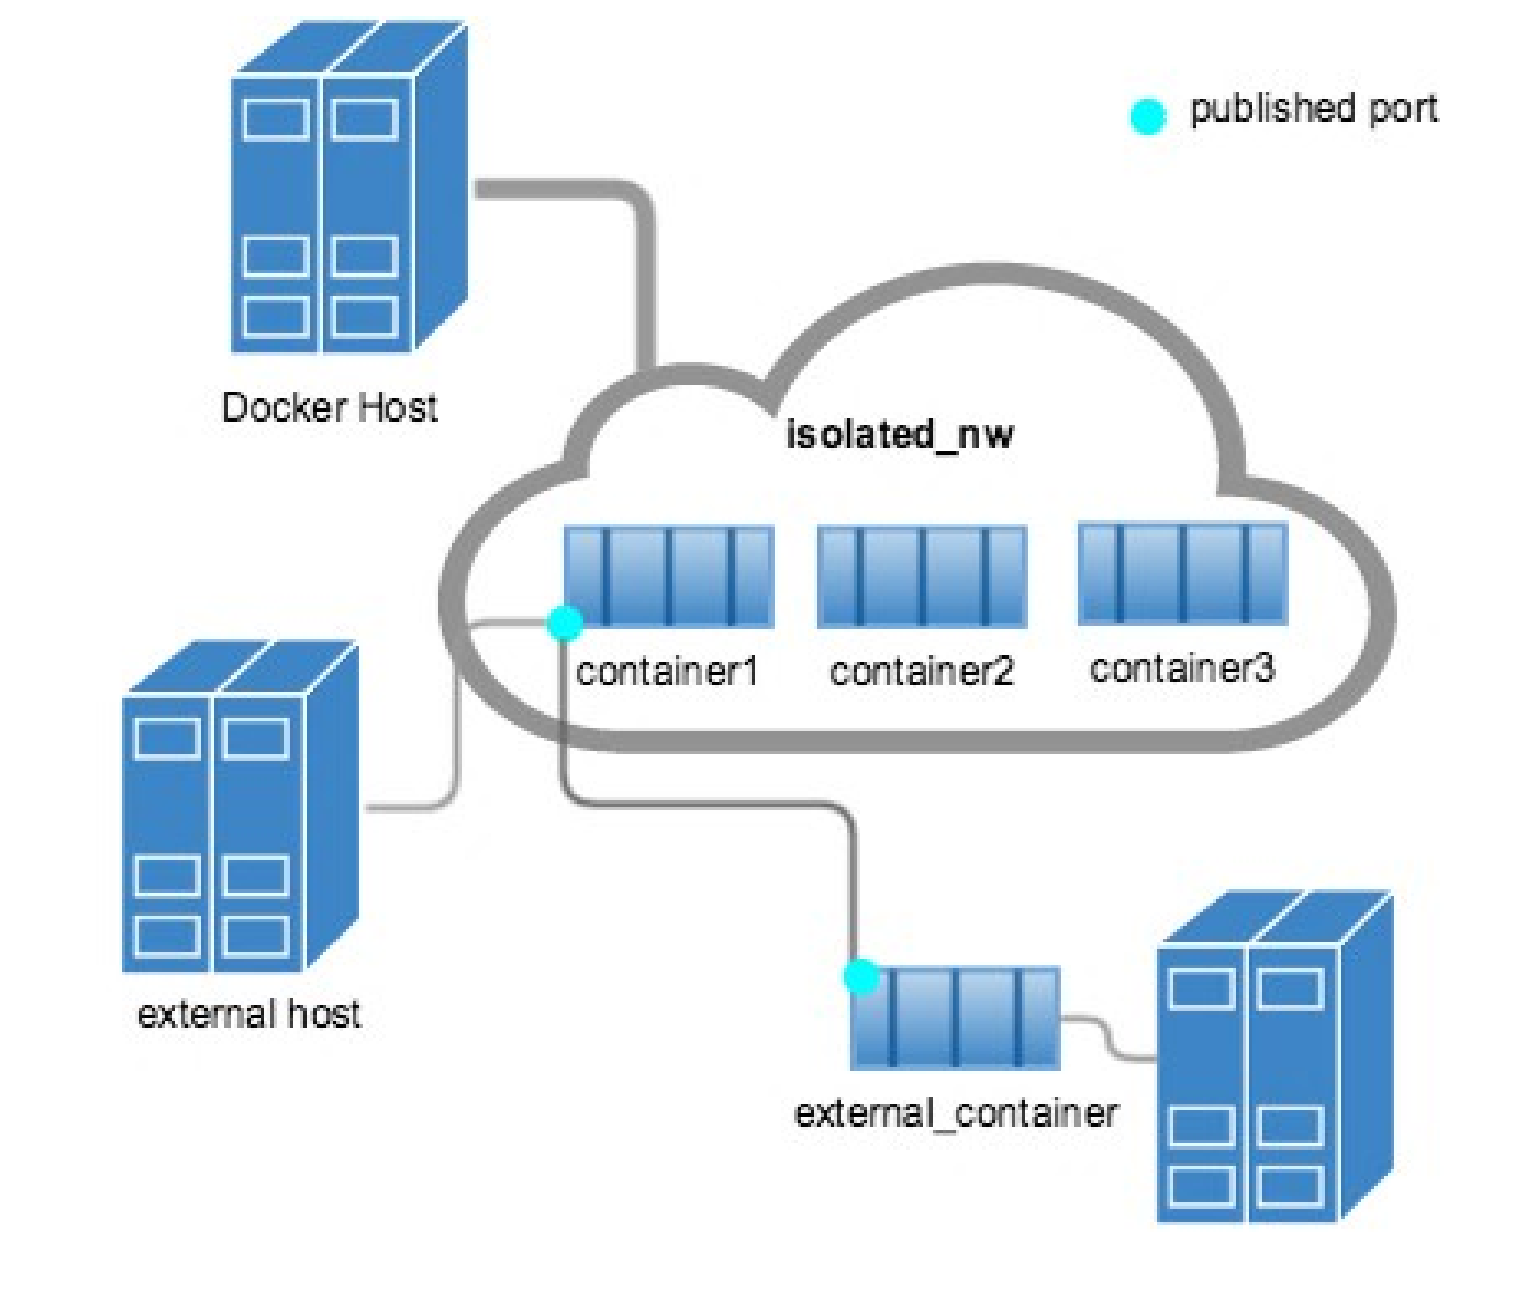
\includegraphics[width=0.7\linewidth]{figures/DockerPortPuEx}
	\caption[Docker Netzwerkzugriff]{Diagramm zur Darstellung des Docker Netzwerkzugriffs im User definierten Bridge-Netzwerk}
	\label{fig:dockerportpuex}
	\tiny{\quelle\url{https://docs.docker.com/engine/userguide/networking/}}
\end{figure}

Möchte man nun in einem Default oder User definierten Bridge-Netzwerk eines Host-Systems, wie in Abbildung \ref{fig:dockerportpuex} abgebildet, dass z. B. einzelne Container sich mit einem externem Host oder einem externen Container austauschen können, so ist ein \textit{Port exposing} und \textit{Publishing} notwendig.
Das \textit{Port exposing} erfolgt entweder durch Eintragung einer beliebigen Portnummer in Kombination mit dem Schlüsselwort \textbf{EXPOSE} im Dockerfile oder durch Ergänzung des \textit{docker run} Kommandos mit dem Flag \textit{{-}{-}expose}.

Für das \textit{Publishing} ist das Festlegen eines Ports im Dockerfile nicht möglich.
Stattdessen wird das \textit{docker run} Kommando durch das Flag \textit{{-}{-}publish} oder \textit{{-}{-}publish-all} ergänzt.
Dies teilt mit, welcher Port $>30000$ auf dem Host-System verfügbar ist.
Möchte man dennoch einen speziellen Port verwenden, so ist die Zuweisung des Ports erst zur Laufzeit möglich.

Aufgrund dessen, dass User definierte Bridge-Netzwerke vorrangig dafür verwendet werden kleinere Netzwerke auf einem Host zu erstellen, eignet sich diese Netzwerklösung nicht zur Umsetzung des Themas.
Dies liegt daran, dass Docker für diese Arbeit im Swarm Modus genutzt wird.
Hierbei handelt es sich um ein Cluster aus mehreren Docker-Engines.
Das Cluster besitzt mindestens einen Swarm-Manager.
Dieser nimmt Befehle für den Swarm entgegen und ermöglicht es, neue Swarm-Nodes, auch Swarm-Worker genannt, aber keine einzelnen Docker-Container zum Cluster hinzuzufügen.

Statt des User definierten Bridge-Netzwerks bietet Docker hierfür die Möglichkeit zur Erstellung eines Overlay-Netzwerks auf einem Swarm-Manager an.
Hierbei wird automatisch die Netzwerkbrücke \textit{docker\_gwbridge}, die zur Kommunikation zwischen den Swarm-Nodes verwendet wird, erstellt.
Diese Netzwerkbrücke wird zusätzlich immer dann angelegt, wenn ein gewöhnlicher Docker-Container keine Anbindung an ein externes Netz besitzt.
Der Swarm-Manager gewährt den einzelnen Swarm-Workern immer dann den Zugriff auf das Netzwerk, wenn die Swarm-Worker das Netzwerk zur Bewältigung ihrer Aufgaben benötigen. 

Bei der Erstellung des Overlay-Netzwerks ist zu beachten, dass die Docker-Engine im Swarm Modus arbeitet und der gewählte Swarm-Manager nicht an einen externen Key-Value-Store, wie z. B. ZooKeeper, angebunden ist.

Andernfalls spricht man von einem Overlay-Netzwerk ohne Swarm Modus.
Dieses wird in dieser Arbeit nicht weiter erläutert.
Einerseits, da es nicht erforderlich ist und andererseits, da Docker Inc. hierzu folgenden Satz in ihrem \glqq{}Docker container networking Guide\grqq{} verfasste:

\begin{quote}
	\textit{\glqq{}It may be deprecated in the future \cite{Docker:online3}.\grqq{}}
\end{quote}

\subsection{Volumes und shared Volumes}
\label{ss:sharedVolumes}
Wie bereits im Unterkapitel \ref{c:einführung} erwähnt, werden per default die Daten eines Containers in die writable Schicht des Docker-Containers geschrieben. 
Neben dem Nachteil, dass dieses Vorgehen die Container vergrößert, sind die darin abgelegten Daten lediglich zur Laufzeit des Containers verfügbar und werden nach der Ausführung gelöscht.

\begin{figure}
	\centering
	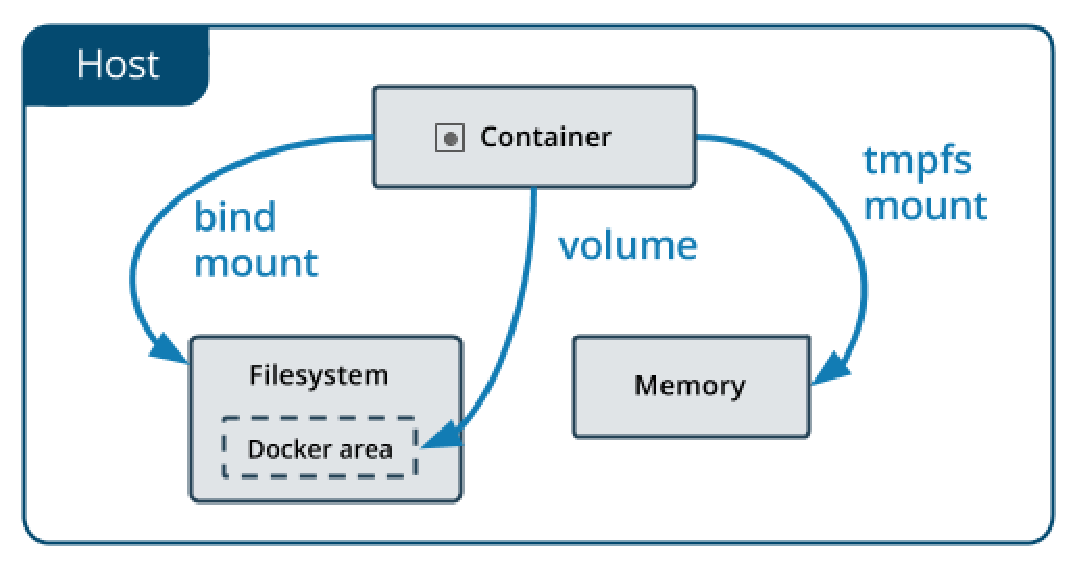
\includegraphics[width=0.7\linewidth]{figures/DockerMounts}
	\caption[Docker Mount Typen]{Übersicht der von Docker gebotenen Mount Typen}
	\label{fig:dockermounts}
	\tiny{\quelle\url{https://docs.docker.com/engine/admin/volumes/}}
\end{figure}

Aufgrund dessen bietet Docker zur dauerhaften Sicherung der Daten eines Containers, wie in Abbildung \ref{fig:dockermounts} gezeigt, die Verwendung von \textit{bind mounts}, \textit{tempfs mounts} und \textit{volumes} an.

Hierbei ist einerseits zu beachten, dass \textit{tempfs mount} vorrangig für Anwendungen mit hoher Performance oder sicherheitskritischen Daten genutzt wird und andererseits, dass Docker die Verwendung von \textit{bind mounts} in ihrer Dokumentation im Unterkapitel \glqq{}Use bind mounts\grqq{} für neu erstellte Anwendungen nicht empfiehlt. 
Somit wird lediglich die Datenspeicherung mit Hilfe von Volumes für die Anwendung verwendet und betrachtet.

Neben den Möglichkeiten zur Datensicherung geht aus Abbildung \ref{fig:dockermounts} hervor, dass das Volume in das Dateisystem eines Docker-Containers, im Swarm-Modus auch als Service bezeichnet, gemounted und der Inhalt auf dem Host-System (Windows oder Unix) gespeichert wird. 
Die Verwaltung des Volumes erfolgt entweder mittels des Docker \ac{CLI} oder der Docker API.

Aufgrund der Anforderung, dass die beiden erzeugten Volumes künftig von mehreren Services genutzt, beschrieben, gelesen und auf einem eigenen Host-System laufen sollten, konnten weder read-only noch lokale Volumes verwendet werden. 
Stattdessen wurden zwei shared Volumes durch Verwendung eines Volume Treibers realisiert.

Hierfür ist das Docker NFS, AWS EFS \& Samaba/CIFS Volume Plugin auf einem eigenen Host-System installiert worden.
Mit diesem wurde das Volume \textit{gatling-logs} erzeugt, das anschließend zu den Attack-Nodes und dem Reporter-Node der Anwendung gemountet wurde. 
Zusätzlich zum \textit{gatling-logs} ist das \textit{gatling-results} Volume erstellt worden. 
Dieses wurde im Reporter-Node und dem Report-Viewer Node des Swarms gemountet.

Somit verfügt der Reporter-Node über alle Daten des Angriffs und leitet diese per \textit{gatling-results} Volume an den Reporter-Viewer-Node, der für die Verwertung der Ergebnisse zuständig ist, weiter.

\chapter{Gatling - Testing Framework}

In diesem Kapitel soll auf das Testing Framework \textit{Gatling.io} eingegangen werden. Im Besonderen wird analysiert, was Performance-Tests sind und welche Vorteile diese für den Entwickler bzw. die Softwarearchitektur mit sich bringen.
\newline
Nachdem mögliche Einsatzgebiete von Performance-Tests analysiert wurden, wird auf die \ac{DSL} von Gatling.io eingegangen. Es werden hier die wichtigsten Befehle erläutert.

%https://gatling.io/

\section{Performance-Tests}

Performance Tests sind für jede größere Anwendung von essentieller Bedeutung. Durch diese Art der Tests können sogenannte \textit{Bottlenecks} der Anwendung ausfindig gemacht und beseitigt werden. Unter den \textit{Bottlenecks} versteht man einzelne Komponenten der programmierten Anwendung, die den gesamten Worfklow ausbremsen. Als Beispiel könnte folgende Situation dienen:
\begin{itemize}
    \item Eine aufwendigere Berechnung wurde in parallele Tasks ausgelagert
    \item Jeder der Tasks muss eine Datenbankabfrage durchführen um die aktuellsten Daten zur Verfügung zu haben
    \item Durch diese langwierige Abfrage verzögert sich die gesamte Berechnung
\end{itemize}
Als Bottleneck ist hier die Abfrage zur Datenbank aufzuführen, diese sollte in einen vorgelagerten Prozess abgespalten werden. Auch wenn dieses konstruierte Beispiel sehr einfach und überzogen dargestellt ist, gibt es in echten Anwendungen auch Problembereiche, die vom Entwickler nicht als solche identifiziert werden konnten. Beispielsweise könnte eine Abfrage an eine Schnittstelle unter normalen Bedingungen sofort erledigt sein, unter Last allerdings ändert sich dessen Verhalten. Ohne einen Test, der eine konstruierte Last bzw. Auslastung auf der Anwendung erzeugt, wird diese Art von Fehler nicht entdeckt. Der Administrator kann so im Vornherein die Infrastruktur anpassen, bevor die Anwendung im produktiven Umfeld ist.
 
\subsection{Einsatzgebiete}

\begin{itemize}
    \item Vorhersage von Bottlenecks in Anwendung:
    
    Durch einen Test, der eine simulierte Auslastung auf der Anwendung erzeugt, können einzelne Problembereiche der Anwendung aufgezeigt werden.
    \item Skalierung der Anwendung:

    Durch Performance-Tests kann eine beliebige Anzahl an Usern auf der Anwendung simuliert werden. Es könnte beispielsweise die Skalierung der Anwendung erprobt werden. Hier wird nicht nur die Softwarearchitektur der Anwendung getestet, sondern auch die IT- Infrastruktur. Durch die genannten Tests könnte beispielsweise aufkommen, dass ein Load-Balancer für eine erwartete Last von 1 Million Benutzern nicht ausreichend ist.
    \item Benutzer Bedienung verbessern -- Latenz Zeiten verringern = schnelleres Feedback für den User
    \item langfristig Verbesserung / Optimierung der Software Architektur  --> wie gut skaliert die Anwendung?

\end{itemize}


\section{DSL}

%https://gatling.io/docs/current/cheat-sheet/

\subsection{Wichtige Befehle}

%Tabelle mit wichtigsten Befehlen zeigen


\section{Metriken}

Welche Metriken sind verfügbar ?
Wie werden diese gesammelt?
Wie werden diese interpretiert?




\section{Continous Integration}

Wie kann Gatling in den bestehenden / zukünftigen Continous Integration Prozess eingebunden werden?

Beispielhaft Jenkins auf Hersteller-seite vorgestellt.


\section{Tests}
In diesem Unterkapitel soll auf den grundsätzlichen Aufbau eines Gatling Tests eingangen werden.\\
Gatling Tests sind in der Programmiersprache Scala\footnote{{} Scala ist eine Java-ähnliche Sprache, die auf der \ac{JVM} läuft.} implementiert.
Im Code-Beispiel \ref{testCodingSample} ist beispielhaft ein solcher Test dargestellt. Dieser soll die Schnittstelle für das zufällige Abholen eines Witzes auf Last testen. Die grundsätzliche Funktionsweise der Schnittstelle wird an dieser Stelle vorausgesetzt. Dies muss im Vornherein durch Unit - bzw. Integrationstests sichergestellt werden. Für das Testen der Auslastung müssen allerdings einige Details über die Schnittstelle bekannt sein. So muss u.a. der Server mit zugehörigem Port, sowie der genaue Aufbau der Schnittstelle für den Entwickler einsehbar sein. Dieser Aspekt wird an dieser Stelle erwähnt, da es in größeren Unternehmen durchaus sein könnte, dass unabhängige Teams die gleiche Anwendung testen müssen. In diesem Fall hätte der Entwickler des Performance-Tests, nur die Black-Box-Sicht auf die bereits programmierte Anwendung. 

Zuerst werden die notwendigen Bibliotheken über \glqq Import-Befehle\grqq{} geladen.  

\begin{minipage}{\linewidth}
\begin{lstlisting}[frame=single,caption=Testabfrage auf Schnittstelle, label=testCodingSample, language=Scala]
import io.gatling.core.Predef._
import io.gatling.http.Predef._
import scala.concurrent.duration._

class RandomJokeSimulation extends Simulation {
    val httpConf = http
        .baseURL("http://192.168.111.20:58080")
        .acceptHeader("application/json")
        .acceptEncodingHeader("gzip, deflate")
        .userAgentHeader("Mozilla/5.0 (Windows NT 5.1; rv:31.0) Gecko/20100101 Firefox/31.0")

    val scn = scenario("RandomJokeSimulation").repeat(100) {
        exec(http("getRandomJoke")
        .get("/api/v1/joke/random"))
    }    

    setUp(
        scn.inject(atOnceUsers(100))
    ).protocols(httpConf)
}
\end{lstlisting}
\end{minipage}



Unterschiede Lasttests zu Unit / Integrationtests usw.
%https://jaxenter.de/mit-dem-testen-von-anwendungen-ist-es-so-eine-last-erst-recht-mit-lasttests-27564



Allgemein Alternative mit JMeter
%https://www.heise.de/developer/artikel/Last-und-Performance-Tests-mit-JMeter-oder-Gatling-3648505.html

JMeter vs Gatling
%https://octoperf.com/blog/2015/06/08/jmeter-vs-gatling/


\section{Zwischenfazit Lasttests}

Performance oder Lasttests sind notwendig um eine stabile Anwendung bzw. API zu erreichen.
Langfristig wird sich die Architektur bzw. der Programmierprozess verbessern wenn die Ergebnisse der Tests analysiert, ausgewertet und auch für zukünftige Entwicklung berücksichtigt werden.



\chapter{Kubernetes}

\section{Einführung}

\section{Architektur}

\section{Skalierung}

\section{Persistenz}

\section{Service Discovery und Load Balancing}

\section{Batch Exectution}
\chapter{Java Vert.x}

\section{Reaktive Programmierung}

\subsection{Konzepte}

\section{Skalierung}

\section{Einsatzgebiete}


\chapter{Fazit}

\section{Eignung von Container getriebenen Lasttests}
\label{s:conclusionContainerDrivenStressTests}

Als Fazit l\"asst sich festhalten, dass Lasttests mit Gatling und Docker durchaus m\"oglich sind, allerdings muss die statistische Aussagekraft mit einiger Skepsis betrachtet werden.
Die in Abschnitt~\ref{s:valuationProblems} beschriebenen Probleme im Startverhalten sorgen daf\"ur, dass einige Kenngr\"o\ss{}en als eher unzuverl\"assig zu betrachten sind.

Um diese Probleme zu beheben, m\"usste man ein Synchronisierungsverfahren entwickeln, das sicherstellt, dass alle Attack-Container erst dann mit der Simulation beginnen, wenn alle anderen Attack-Container auch verf\"ugbar sind.
Im Prinzip geht es dabei um eine Art invertierten Semaphor, der daf\"ur sorgt, dass alle beteiliten Parteien nur gemeinsam den kritischen Abschnitt betreten.

Eine primitive Implementierung k\"onnte man bspw. durch eine Kombination von Lock-Dateien und Busy-Waiting umsetzen.
Der Vorteil dieser Variante ist, dass man diese auch noch durch Bash-Skripte umsetzen kann.

Eine weitere M\"oglichkeit zur Implementierung w\"are die Nutzung von Linux-Pipes.
Daf\"ur m\"usste man aber bereits einen Control Container nutzen, der eine \glqq{}Registration-Pipe\grqq{} und eine \glqq{}Notify-Pipe\grqq{} bereitstellt.
Anschlie\ss{}end k\"onnten sich alle Attack-Container an der \glqq{}Registration-Pipe\grqq{} melden und danach an der \glqq{}Notify-Pipe\grqq{} lauschen, bis alle Attack-Container sich registriert haben, um erst dann zu starten.

Beide Verfahren w\"urden die Zeitdifferenz zwischen den Simulationsstarts vermutlich immerhin auf $\pm 1s$ senken.
Allerdings lassen sich dadurch leichte Unterschiede bspw. bei der Kompilierungszeit der Scenarios immer noch nicht kontrollieren.
Eine genauere Synchronisierung ist nur innerhalb der Lasttest-Anwendung m\"oglich.
So k\"onnte man alle Instanzen dieser abstrakten Anwendung z. B. \"uber einen Message Bus synchronisieren.
Leider bietet Gatling offenbar keine M\"oglichkeit eine solche Synchronisierung durchzuf\"uhren.
Zumindest ist in der Dokumentation nichts dazu zu finden.

Unabh\"angig von der statistischen Aussagekraft der Ergebnisse sind Lasttests mit Gatling und Docker dennoch eine sehr gute M\"oglichkeit, um eine Anwendung an die Grenze der Belastbarkeit und dar\"uber hinaus zu bringen.
Dies ist speziell dann von Interesse, wenn man herausfinden will, wann die Software sprichw\"ortlich \glqq{}zusammenbricht\grqq{}.
Also zum Beispiel die Success-Error-Rate stark abnimmt, weil der HTTP-Timeout von 60s immer \"ofter erreicht wird.

Auch f\"ur die Untersuchung der Skalierbarkeit der Anwendung sind Lasttests mit Docker sehr geeignet.
So kann unter der Voraussetzung, dass die eigene Anwendung entweder bereits als Docker Image vorliegt oder mit vertretbarem Aufwand zu einem Image paketiert werden kann, sehr anschaulich getestet werden, ob die horizontale Skalierung einer Komponente (z. B. eines einzelnen Microservices) tats\"achlich der Durchsatz dieser oder abh\"angiger Komponenten im selben Ma\ss{} gesteigert werden kann oder ob daf\"ur ggf. weitere Schritte notwendig sind.

Als letzter Punkt sei genannt, dass Docker getriebene Lasttests einen weiteren eminenten Vorteil gegen\"uber klassischen Lasttests haben, da sie durch die Verteilung der Container auch die Latenz des Netzwerks st\"arker ber\"ucksichtigen.
So ist der maximal erzeugbare Netzwerktraffic nicht mehr abh\"angig von der Bandbreite, die ein einzelner Host bereitstellen kann.
Sowohl die beiden vorgestellten Clustermanagementsysteme Kubernetes (vgl. Kapitel~\ref{c:kubernetes}) und Docker Swarm (vgl. Kapitel~\ref{c:docker}) als auch alle anderen weiter verbreiteten Systeme wie DC/OS Mesos u. Marathon sind daf\"ur optimiert, die Last auf alle Knoten des Clusters zu verteilen, wodurch nat\"urlich auch die Gesamtbandbreite vergr\"o\ss{}ert wird (zumindest solange sich die Anwendungs-Container und Lasttest-Container im selben Netzwerk-Segment befinden und nicht z. B. durch eine Firewall ausgebremst werden).

\section{Ausblick}

Bei einer Weiterf\"uhrung des Projekts g\"alte es einerseits, falls erforderlich, die in den Abschnitten~\ref{s:valuationProblems} und \ref{s:conclusionContainerDrivenStressTests} angesprochenen Probleme und L\"osungsans\"atze zu verfolgen, um die statistische Aussagekr\"aftigkeit der Tests zu erh\"ohen.
Andererseits k\"onnte man die bereits existierenden Konfigurationen f\"ur Docker-Compose und Docker Swarm um Konfigurationen f\"ur Kubernetes bzw. OpenShift erg\"anzen, da sich diese im Enterprise Sektor deutlich gr\"o\ss{}erer Beliebtheit erfreuen als Docker Swarm.
Die notwendigen Grundlagen daf\"ur wurden in Kapitel~\ref{c:kubernetes} bereits erl\"autert.
So k\"onnten in Kubernetes die Szenario-Dateien auch in einem Cluster-Szenario durch das Feature \glqq{}Persistent Volumes\grqq{} den Attack-Container bekannt gemacht werden.
Ein \"Aquivalent zur Docker Swarm Config API w\"are die Speicherung der Simulationsdateien in \textit{etcd}, wobei hier die Variante der Persistent Volumes klar zu favorisieren ist.

Ein weiterer Gesichtspunkt der bereits etwas ausgereifteren Clustermanagementsysteme ist die bereits angesproche automatische Skalierung.
Auch hier k\"onnten Container getriebene Lasttests von Interesse sein, wenn es darum geht Thresholds f\"ur das Up- und Downscaling zu validieren.
Zudem ist es auch wichtig zu testen, wie schnell sich ein zus\"atzlich gestarteter Container im Antwortverhalten bemerkbar macht.
Eine Schwierigkeit hierbei ist, dass mehrere Komponenten ineinander greifen und sich ggf. nicht klar bestimmen l\"asst, welche Komponente nun tats\"achlich das \glqq{}Bottleneck\grqq{} ist. In Frage kommen unter anderem Warm-Up-Time des Containers (wie lange braucht ein Container um Anfragen beantworten zu k\"onnen), Load Balancer (wie schnell wird ein neu gestarteter Container im Load Balancing ber\"ucksichtigt) oder auch, ob \"uberhaupt die richtige Komponente skaliert wurde oder ob das Problem urspr\"unglich von einer anderen Komponente r\"uhrt.



\appendix
\chapter*{Abkürzungen}
\begin{acronym}
\acro{DSL}{Domain Specific Language} 
\acro{GUI}{Graphical User Interface}
\acro{HTTP}{Hypertext Transfer Protocol} 
\acro{JVM}{Java Virtual Maschine} 
\acro{REST}{Representational State Transfer} 
\acro{TFS}{Team Foundation Server}
\acro{URI}{Uniform Resource Identifier}
\acro{VM}{Virtual Machine}
\acro{cgroups}{Control Groups}
\acro{UnionFS}{Union File System}
\acro{DDC}{Docker Datacenter}
\acro{CLI}{Command-line Interface}
\end{acronym}

\chapter{Anhang}
%Do not display source code chapters in toc
\addtocontents{toc}{\protect\setcounter{tocdepth}{0}}


\addtocontents{toc}{\protect\setcounter{tocdepth}{2}}

\chapter{Verzeichnisse}
\listoffigures
\cleardoublepage
\lstlistoflistings
\cleardoublepage
\listoftables
\cleardoublepage



\bibliographystyle{natger}
\bibliography{thesis}

\footnotesize


\end{document}
